% Options for packages loaded elsewhere
\PassOptionsToPackage{unicode}{hyperref}
\PassOptionsToPackage{hyphens}{url}
\PassOptionsToPackage{dvipsnames,svgnames,x11names}{xcolor}
%
\documentclass[
  letterpaper,
  DIV=11,
  numbers=noendperiod]{scrartcl}

\usepackage{amsmath,amssymb}
\usepackage{iftex}
\ifPDFTeX
  \usepackage[T1]{fontenc}
  \usepackage[utf8]{inputenc}
  \usepackage{textcomp} % provide euro and other symbols
\else % if luatex or xetex
  \usepackage{unicode-math}
  \defaultfontfeatures{Scale=MatchLowercase}
  \defaultfontfeatures[\rmfamily]{Ligatures=TeX,Scale=1}
\fi
\usepackage{lmodern}
\ifPDFTeX\else  
    % xetex/luatex font selection
\fi
% Use upquote if available, for straight quotes in verbatim environments
\IfFileExists{upquote.sty}{\usepackage{upquote}}{}
\IfFileExists{microtype.sty}{% use microtype if available
  \usepackage[]{microtype}
  \UseMicrotypeSet[protrusion]{basicmath} % disable protrusion for tt fonts
}{}
\makeatletter
\@ifundefined{KOMAClassName}{% if non-KOMA class
  \IfFileExists{parskip.sty}{%
    \usepackage{parskip}
  }{% else
    \setlength{\parindent}{0pt}
    \setlength{\parskip}{6pt plus 2pt minus 1pt}}
}{% if KOMA class
  \KOMAoptions{parskip=half}}
\makeatother
\usepackage{xcolor}
\usepackage[top=20mm,left=20mm,right=20mm,bottom=20mm]{geometry}
\setlength{\emergencystretch}{3em} % prevent overfull lines
\setcounter{secnumdepth}{5}
% Make \paragraph and \subparagraph free-standing
\makeatletter
\ifx\paragraph\undefined\else
  \let\oldparagraph\paragraph
  \renewcommand{\paragraph}{
    \@ifstar
      \xxxParagraphStar
      \xxxParagraphNoStar
  }
  \newcommand{\xxxParagraphStar}[1]{\oldparagraph*{#1}\mbox{}}
  \newcommand{\xxxParagraphNoStar}[1]{\oldparagraph{#1}\mbox{}}
\fi
\ifx\subparagraph\undefined\else
  \let\oldsubparagraph\subparagraph
  \renewcommand{\subparagraph}{
    \@ifstar
      \xxxSubParagraphStar
      \xxxSubParagraphNoStar
  }
  \newcommand{\xxxSubParagraphStar}[1]{\oldsubparagraph*{#1}\mbox{}}
  \newcommand{\xxxSubParagraphNoStar}[1]{\oldsubparagraph{#1}\mbox{}}
\fi
\makeatother


\providecommand{\tightlist}{%
  \setlength{\itemsep}{0pt}\setlength{\parskip}{0pt}}\usepackage{longtable,booktabs,array}
\usepackage{calc} % for calculating minipage widths
% Correct order of tables after \paragraph or \subparagraph
\usepackage{etoolbox}
\makeatletter
\patchcmd\longtable{\par}{\if@noskipsec\mbox{}\fi\par}{}{}
\makeatother
% Allow footnotes in longtable head/foot
\IfFileExists{footnotehyper.sty}{\usepackage{footnotehyper}}{\usepackage{footnote}}
\makesavenoteenv{longtable}
\usepackage{graphicx}
\makeatletter
\def\maxwidth{\ifdim\Gin@nat@width>\linewidth\linewidth\else\Gin@nat@width\fi}
\def\maxheight{\ifdim\Gin@nat@height>\textheight\textheight\else\Gin@nat@height\fi}
\makeatother
% Scale images if necessary, so that they will not overflow the page
% margins by default, and it is still possible to overwrite the defaults
% using explicit options in \includegraphics[width, height, ...]{}
\setkeys{Gin}{width=\maxwidth,height=\maxheight,keepaspectratio}
% Set default figure placement to htbp
\makeatletter
\def\fps@figure{htbp}
\makeatother

\KOMAoption{captions}{tableheading}
\usepackage{sansmathfonts}
\usepackage[utf8]{inputenc}
\usepackage[T1]{fontenc}
\renewcommand*\familydefault{\sfdefault}
\makeatletter
\@ifpackageloaded{caption}{}{\usepackage{caption}}
\AtBeginDocument{%
\ifdefined\contentsname
  \renewcommand*\contentsname{Table des matières}
\else
  \newcommand\contentsname{Table des matières}
\fi
\ifdefined\listfigurename
  \renewcommand*\listfigurename{Liste des Figures}
\else
  \newcommand\listfigurename{Liste des Figures}
\fi
\ifdefined\listtablename
  \renewcommand*\listtablename{Liste des Tables}
\else
  \newcommand\listtablename{Liste des Tables}
\fi
\ifdefined\figurename
  \renewcommand*\figurename{Figure}
\else
  \newcommand\figurename{Figure}
\fi
\ifdefined\tablename
  \renewcommand*\tablename{Table}
\else
  \newcommand\tablename{Table}
\fi
}
\@ifpackageloaded{float}{}{\usepackage{float}}
\floatstyle{ruled}
\@ifundefined{c@chapter}{\newfloat{codelisting}{h}{lop}}{\newfloat{codelisting}{h}{lop}[chapter]}
\floatname{codelisting}{Listing}
\newcommand*\listoflistings{\listof{codelisting}{Liste des Listings}}
\usepackage{amsthm}
\theoremstyle{definition}
\newtheorem{exercise}{Exercice}[section]
\theoremstyle{definition}
\newtheorem{definition}{Définition}[section]
\theoremstyle{remark}
\AtBeginDocument{\renewcommand*{\proofname}{Preuve}}
\newtheorem*{remark}{Remarque}
\newtheorem*{solution}{Solution}
\newtheorem{refremark}{Remarque}[section]
\newtheorem{refsolution}{Solution}[section]
\makeatother
\makeatletter
\makeatother
\makeatletter
\@ifpackageloaded{caption}{}{\usepackage{caption}}
\@ifpackageloaded{subcaption}{}{\usepackage{subcaption}}
\makeatother

\ifLuaTeX
\usepackage[bidi=basic]{babel}
\else
\usepackage[bidi=default]{babel}
\fi
\babelprovide[main,import]{french}
% get rid of language-specific shorthands (see #6817):
\let\LanguageShortHands\languageshorthands
\def\languageshorthands#1{}
\ifLuaTeX
  \usepackage{selnolig}  % disable illegal ligatures
\fi
\usepackage{bookmark}

\IfFileExists{xurl.sty}{\usepackage{xurl}}{} % add URL line breaks if available
\urlstyle{same} % disable monospaced font for URLs
\hypersetup{
  pdftitle={Mouvement rectiligne uniforme},
  pdflang={fr},
  colorlinks=true,
  linkcolor={blue},
  filecolor={Maroon},
  citecolor={Blue},
  urlcolor={Blue},
  pdfcreator={LaTeX via pandoc}}


\title{Mouvement rectiligne uniforme}
\author{}
\date{}

\begin{document}
\maketitle


\section{Introduction}\label{introduction}

Nous allons réaliser une expérience numérique à partir de l'application
suivante.

\begin{figure}[H]

{\centering 
\includegraphics[width=0.2\textwidth,height=\textheight]{figures/mru/mru-1.pdf}

}

\caption{QR-code de l'application}

\end{figure}%

Sur cette application, on va d'abord observer le mouvement de la voiture
rouge et mesurer la position de cette voiture à 10 moments, en
remplissant le tableau suivant.

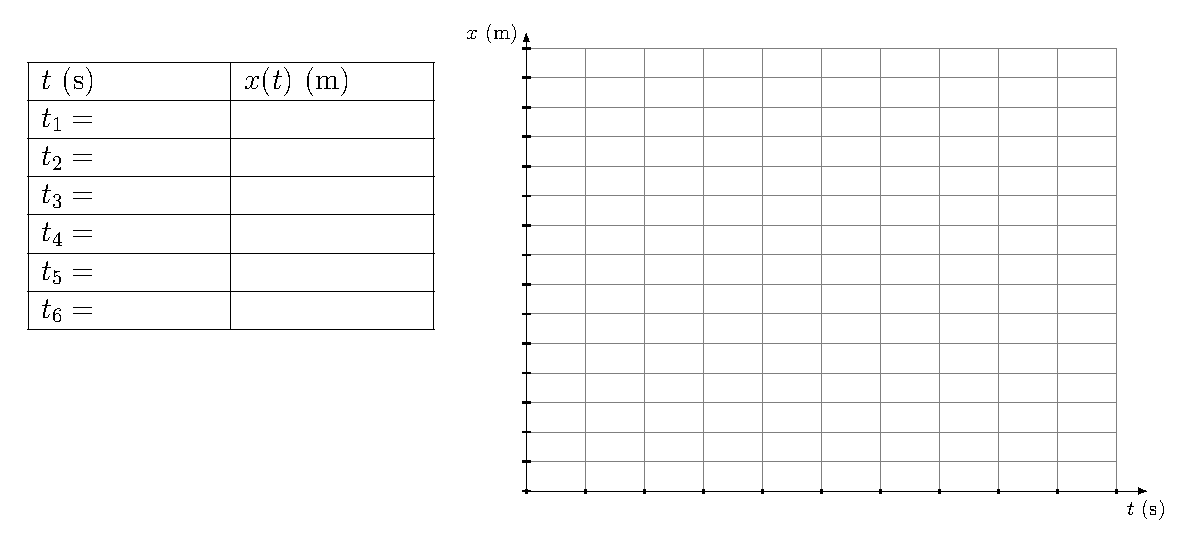
\includegraphics[width=1\textwidth,height=\textheight]{figures/mru/fig2.pdf}

Que constates-tu? \newpage

Calculons maintenant la vitesse moyenne sur différents intervalles de
temps. Pour rappel, la vitesse moyenne entre \(t_0\) et \(t_1\) est
définie par

\[
v_{\text{m}}=\dfrac{\Delta x}{\Delta t}=\dfrac{x(t_1)-x(t_0)}{t_1-t_0}.
\] Autrement dit, la vitesse moyenne entre \(t_0\) et \(t_1\) est la
distance parcourue entre \(t_0\) et \(t_1\) divisée par la durée
\(t_1-t_0\).

Complétons le tableau suivant.

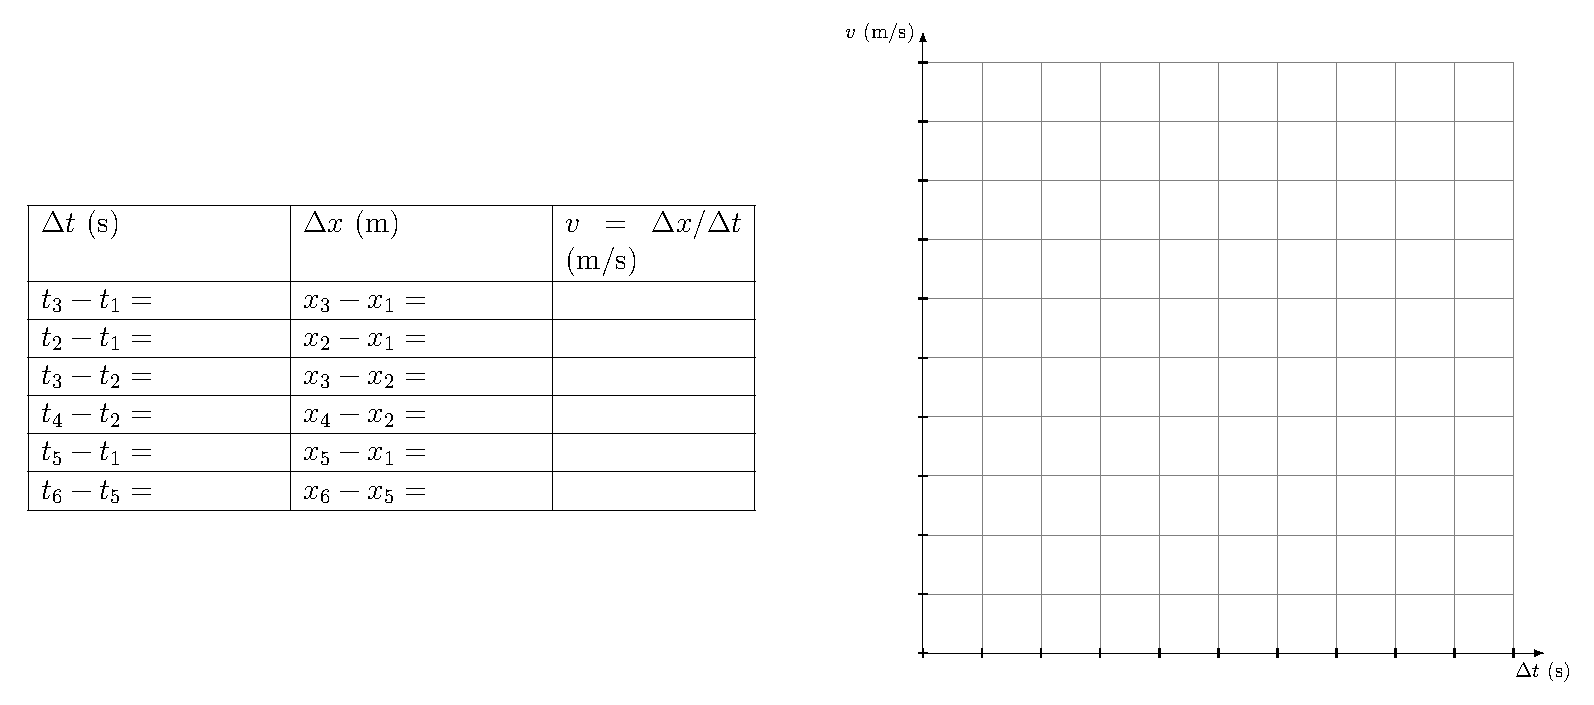
\includegraphics[width=1\textwidth,height=\textheight]{figures/mru/fig3.pdf}

Que constates-tu?

\vspace{3cm}

Nous venons de construire un modèle pour décrire le mouvement effectué
par la voiture. En résumé, le modèle dit ceci:

\begin{enumerate}
\def\labelenumi{\arabic{enumi}.}
\tightlist
\item
  la vitesse de la voiture est constante, pour chaque intervalle de
  temps, la vitesse moyenne. Ici \(v=\)
\item
  la position \(x(t)\) de la voiture en fonction du temps est une
  fonction du premier degré, du type \(x(t)=m\cdot t+p\). De plus,

  \begin{itemize}
  \tightlist
  \item
    l'ordonnée à l'origine est la position initiale: \(x(0)=x_0=\)
  \item
    le taux d'accroissement (=pente de la droite qui représente
    \(x(t)\)) est égal à la vitesse de la voiture. Ainsi, on dispose
    d'une formule pour calculer et représenter la position en fonction
    du temps:
  \end{itemize}

  \[
  x(t)=v\cdot t+x_0=
  \]
\end{enumerate}

Ce modèle permet de faire deux choses importantes:

\begin{enumerate}
\def\labelenumi{\arabic{enumi}.}
\tightlist
\item
  interpoler: grâce à ce modèle, on peut calculer toutes les positions
  entre le moment de départ et le moment où on a arrêté le chronomètre.
\item
  extrapoler: grâce à ce modèle, on peut faire des prédictions.
  Autrement dit, on peut à l'avance connaître la position de la voiture
  à des instants qui sont au delà du temps où on a arrêté le
  chronomètre, pour autant que l'on suppose que la voiture continue sa
  trajectoire sous les mêmes conditions.
\end{enumerate}

Vérifions ces deux affirmations, pour les temps \(t_1=\ldots\ldots\) et
\(t_2=\ldots\ldots\).

\vspace{2cm}

\section{Les caractéristiques d'un
MRU}\label{les-caractuxe9ristiques-dun-mru}

\begin{definition}[]\protect\hypertarget{def-mru}{}\label{def-mru}

Un corps est en \emph{mouvement rectiligne uniforme} s'il parcourt une
ligne droite à vitesse constante, sans changer de sens.

\end{definition}

Les MRU ont les caractéristiques suivantes:

\subsection{Caractéristiques
graphiques}\label{caractuxe9ristiques-graphiques}

\begin{figure}

\begin{minipage}{0.47\linewidth}

\subsection{Position}\label{position}

La représentation de la position en fonction du temps est une droite
oblique: la fonction \(x(t)\) est une fonction du premier degré.
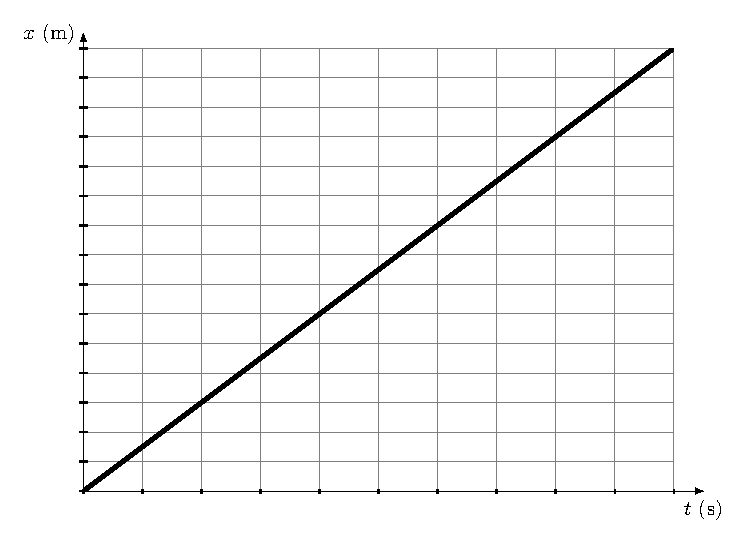
\includegraphics[width=1\textwidth,height=\textheight]{figures/mru/fig4.pdf}\end{minipage}%
%
\begin{minipage}{0.05\linewidth}
~\end{minipage}%
%
\begin{minipage}{0.47\linewidth}

\subsection{Vitesse}\label{vitesse}

La représentation de la vitesse en fonction du temps est une droite
horizontale: la fonction \(v(t)\) est une fonction constante.
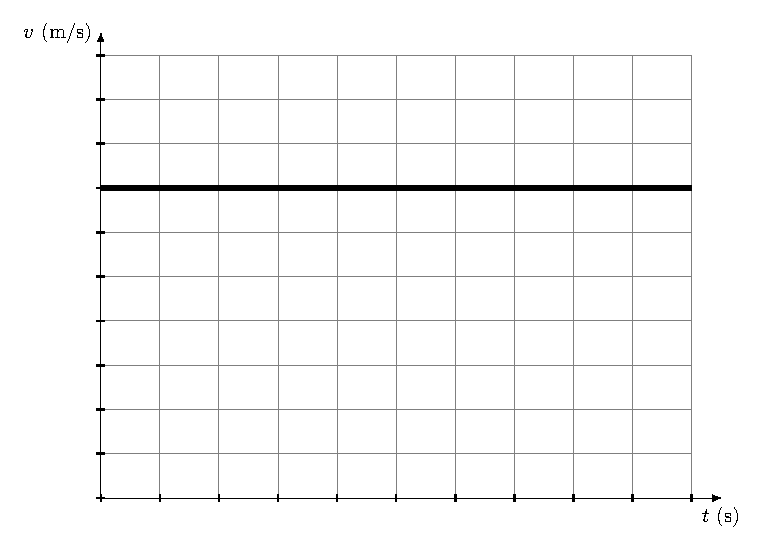
\includegraphics[width=1\textwidth,height=\textheight]{figures/mru/fig5.pdf}\end{minipage}%

\end{figure}%

\subsection{Caractéristiques
analytiques}\label{caractuxe9ristiques-analytiques}

\begin{figure}

\begin{minipage}{0.48\linewidth}

\subsection{Position}\label{position-1}

La position en fonction du temps est donnée par \[
x(t)=v\cdot t+x_0,
\] où \(v\) est la vitesse du corps en MRU et \(x_0\) sa position
initiale.\end{minipage}%
%
\begin{minipage}{0.04\linewidth}
~\end{minipage}%
%
\begin{minipage}{0.48\linewidth}

\subsection{Vitesse}\label{vitesse-1}

La vitesse en fonction du temps est donnée par \[
v(t)=v_{\text{m}}=\text{constante}. 
\]\end{minipage}%

\end{figure}%

\newpage{}

\section{Comparaisons de deux MRU}\label{comparaisons-de-deux-mru}

Revenons à la voiture rouge de l'introduction. Nous allons ajouter une
voiture bleue et observer leurs mouvements, dans deux situations:
lorsqu'elles parcourent la route dans le même sens et lorsqu'elles
parcourent la route dans des sens opposés.

\subsection{Parcours dans le même
sens}\label{parcours-dans-le-muxeame-sens}

\begin{figure}[H]

{\centering 
\includegraphics[width=0.2\textwidth,height=\textheight]{figures/mru/mru-2.pdf}

}

\caption{QR-code de l'application}

\end{figure}%

Tu observes qu'une voiture dépasse l'autre. Comment peux-tu donner le
temps de ce dépassement à l'aide du graphique?

\vspace{3cm}

Quelle voiture va le plus vite? Peux-tu l'observer à l'aide du
graphique?

\vspace{3cm}

\subsection{Parcours dans des sens
opposés}\label{parcours-dans-des-sens-opposuxe9s}

\begin{figure}[H]

{\centering 
\includegraphics[width=0.2\textwidth,height=\textheight]{figures/mru/mru-3.pdf}

}

\caption{QR-code de l'application}

\end{figure}%

Tu observes que les voitures se croisent. Comment peux-tu donner le
temps de ce croisement à l'aide du graphique? \vspace{3cm}

Que vaut la vitesse de la voiture bleue?

\vspace{3cm}

Quelle voiture va le plus vite?

\vspace{3cm}
\newpage

\section{Exercices}\label{exercices}

\begin{exercise}[]\protect\hypertarget{exr-xapdv}{}\label{exr-xapdv}

Sur le graphique ci-dessous, tu as la vitesse, en fonction du temps,
d'un corps en MRU.

\begin{center}
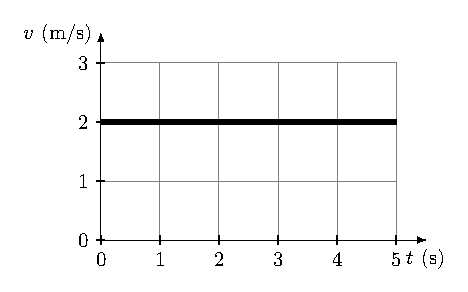
\includegraphics[width=0.4\textwidth,height=\textheight]{figures/mru/fig6.pdf}
\end{center}

Parmi les graphiques ci-dessous, lequel représente la position en
fonction du temps? Explique ton choix. \begin{center}
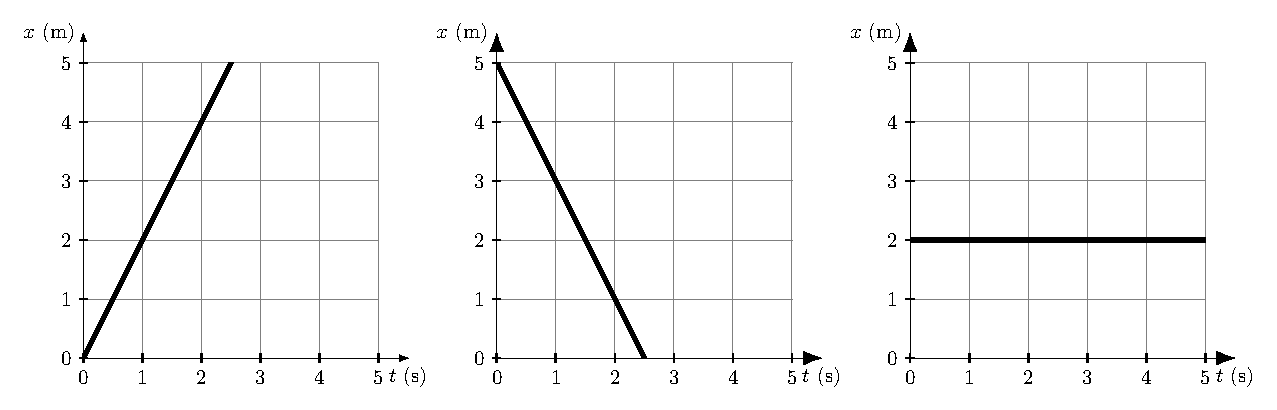
\includegraphics[width=1\textwidth,height=\textheight]{figures/mru/fig7.pdf}
\end{center}

\end{exercise}

\newpage

\begin{exercise}[]\protect\hypertarget{exr-vapdx}{}\label{exr-vapdx}

Sur le graphique ci-dessous, tu as la position, en fonction du temps,
d'un corps en MRU. Trace le graphique de la vitesse de ce corps en
fonction du temps.

\begin{center}
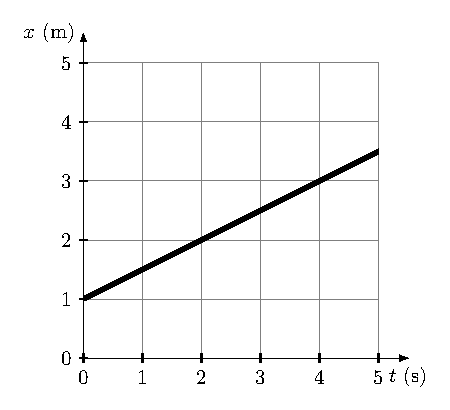
\includegraphics[width=0.4\textwidth,height=\textheight]{figures/mru/fig8.pdf}
\end{center}

\end{exercise}

\begin{exercise}[]\protect\hypertarget{exr-ois}{}\label{exr-ois}

Il y a environ 5km entre le Beffroi de Mons et le centre Sparkoh! Sur
les repères ci-dessous, l'origine correspond au Beffroi. Ces repères
décrivent le mouvement d'oiseaux entre le Beffroi et Sparkoh. Décris ces
mouvement et donne leurs caractéristiques (position initiale, position
finale et vitesse).

\begin{center}
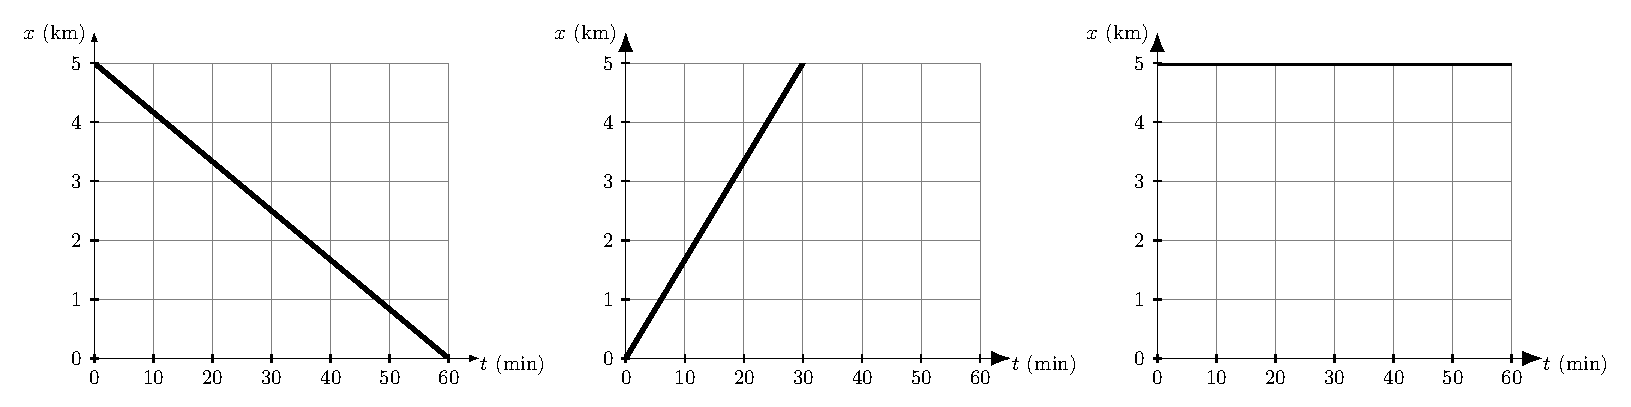
\includegraphics[width=1\textwidth,height=\textheight]{figures/mru/fig9.pdf}
\end{center}

\end{exercise}

\newpage

\begin{exercise}[]\protect\hypertarget{exr-coureur}{}\label{exr-coureur}

Voici le graphique de la position d'un coureur en fonction du temps. Tu
constates que le parcours du coureur peut être décomposé en 5 étapes.
Réponds aux questions suivantes.

\begin{center}
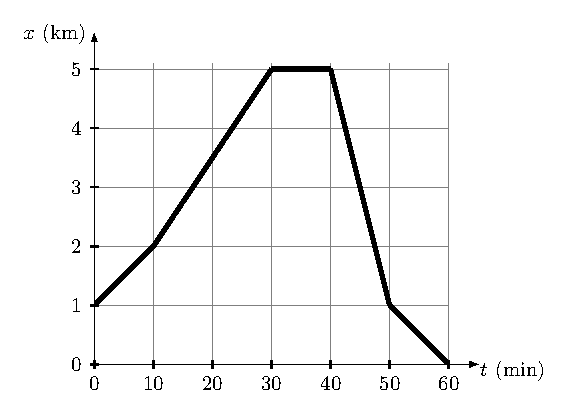
\includegraphics[width=0.5\textwidth,height=\textheight]{figures/mru/fig10.pdf}
\end{center}

Durant quelle(s) étape(s):

\begin{enumerate}
\def\labelenumi{\arabic{enumi}.}
\tightlist
\item
  sa vitesse est positive?
\item
  sa vitesse est négative?
\item
  sa vitesse est nulle?
\item
  sa vitesse est la plus grande, en valeur absolue?
\item
  la distance parcourue est la plus grande?
\item
  la distance parcourue est la plus petite?
\end{enumerate}

\end{exercise}

\begin{exercise}[]\protect\hypertarget{exr-croisement}{}\label{exr-croisement}

Trois particules (A, B et C) se déplacent sur la même droite, comme
indiqué sur le graphique ci-dessous.

\begin{center}
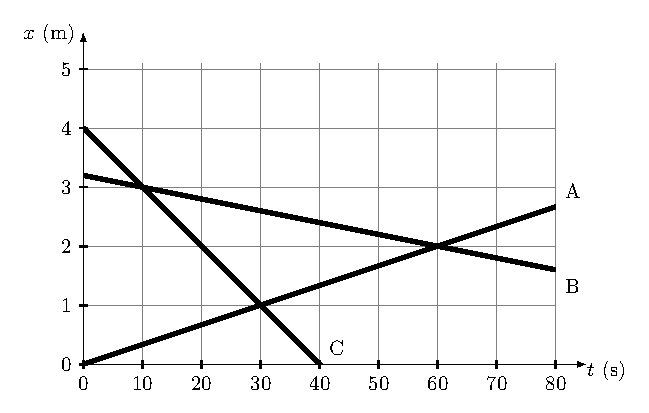
\includegraphics[width=0.5\textwidth,height=\textheight]{figures/mru/fig11.pdf}
\end{center}

Indique si les propositions suivantes sont vraies ou fausses. Justifie.

\begin{enumerate}
\def\labelenumi{\arabic{enumi}.}
\tightlist
\item
  Les trois particules se déplacent dans le même sens.
\end{enumerate}

\vspace{2cm}

\begin{enumerate}
\def\labelenumi{\arabic{enumi}.}
\setcounter{enumi}{1}
\tightlist
\item
  La particule A est la plus rapide.
\end{enumerate}

\vspace{2cm}

\begin{enumerate}
\def\labelenumi{\arabic{enumi}.}
\setcounter{enumi}{2}
\tightlist
\item
  A dépasse C à l'instant \(t=30\text{s}\).
\end{enumerate}

\vspace{2cm}

\begin{enumerate}
\def\labelenumi{\arabic{enumi}.}
\setcounter{enumi}{3}
\tightlist
\item
  B dépasse A à l'instant \(t=60\text{s}\).
\end{enumerate}

\vspace{2cm}

\begin{enumerate}
\def\labelenumi{\arabic{enumi}.}
\setcounter{enumi}{4}
\tightlist
\item
  A est moins rapide que B, à l'instant \(t=60\text{s}\).
\end{enumerate}

\vspace{2cm}

\begin{enumerate}
\def\labelenumi{\arabic{enumi}.}
\setcounter{enumi}{5}
\tightlist
\item
  B est plus près de A que de C, à l'instant \(t=10\text{s}\).
\end{enumerate}

\vspace{2cm}

\begin{enumerate}
\def\labelenumi{\arabic{enumi}.}
\setcounter{enumi}{6}
\tightlist
\item
  C ne croise jamais A.
\end{enumerate}

\vspace{2cm}

\begin{enumerate}
\def\labelenumi{\arabic{enumi}.}
\setcounter{enumi}{7}
\tightlist
\item
  C croise B à deux moments.
\end{enumerate}

\vspace{2cm}

\end{exercise}

\newpage

\begin{exercise}[]\protect\hypertarget{exr-calcul-2}{}\label{exr-calcul-2}

Observe le graphique suivant. Calcule sur base du graphique la vitesse
du corps en mouvement, ainsi que sa position initiale. Donne ensuite une
équation pour \(x(t)\) et \(v(t)\).

\begin{center}
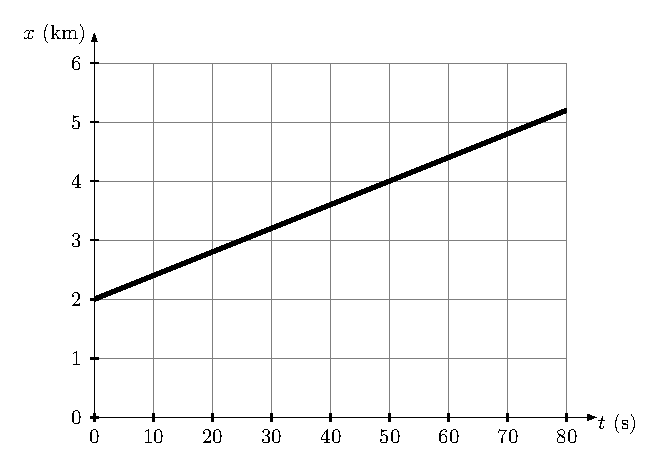
\includegraphics[width=0.5\textwidth,height=\textheight]{figures/mru/fig12.pdf}
\end{center}

\end{exercise}

\vspace{5cm}

\begin{exercise}[]\protect\hypertarget{exr-calcul-1}{}\label{exr-calcul-1}

Un élève de Bervoets longe le hall sportif à vitesse constante. Il longe
l'entiereté du hall en 2 minutes. Sachant que le hall a une longueur de
90m, donne une formule pour la position de cet élève en fonction du
temps. A quel moment aura-t-il parcouru 60m?

\end{exercise}




\end{document}
